\documentclass[../main.tex]{subfiles}
\begin{document}
\subsection{Quantitative as Categorical}

\subsubsection{Radial Visualizations}
\begin{figure}
    \begin{subfigure}{\textwidth}
    \centering
    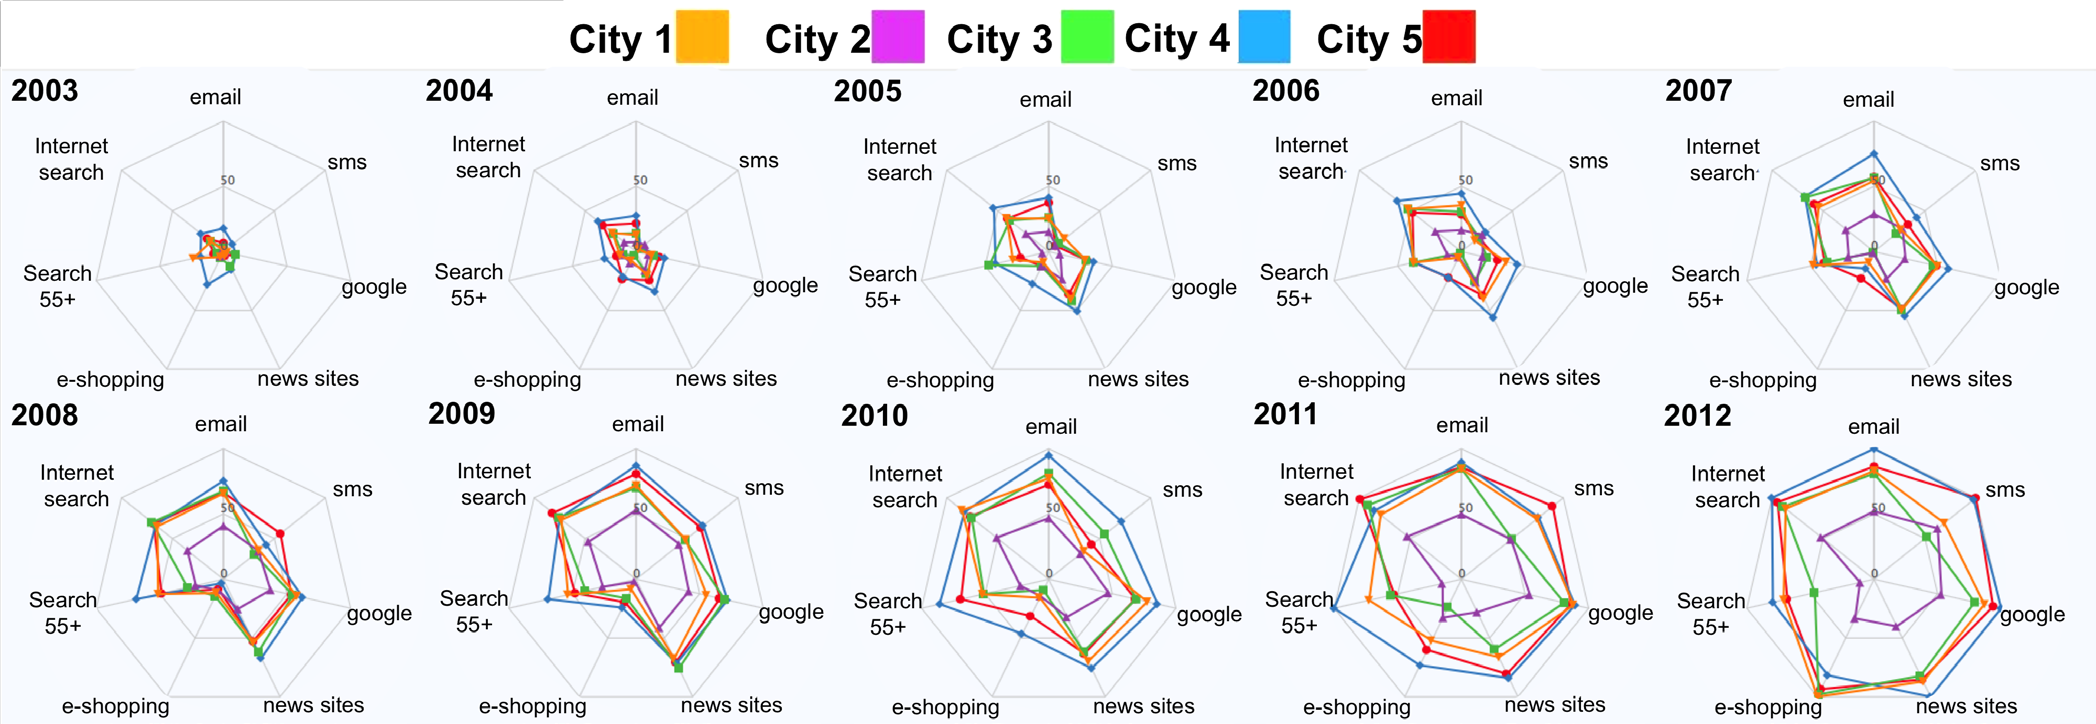
\includegraphics[scale=0.2]{cities.png}
    \caption{The size and shape of each polygon acts as an indicator of Internet usage over time. All events in all cities seem to have expanded over time, indicating a conditional dependence on time.}
    \label{fig:radarchart}
    \end{subfigure}

    \bigskip
    \begin{subfigure}{\textwidth}
    \centering
    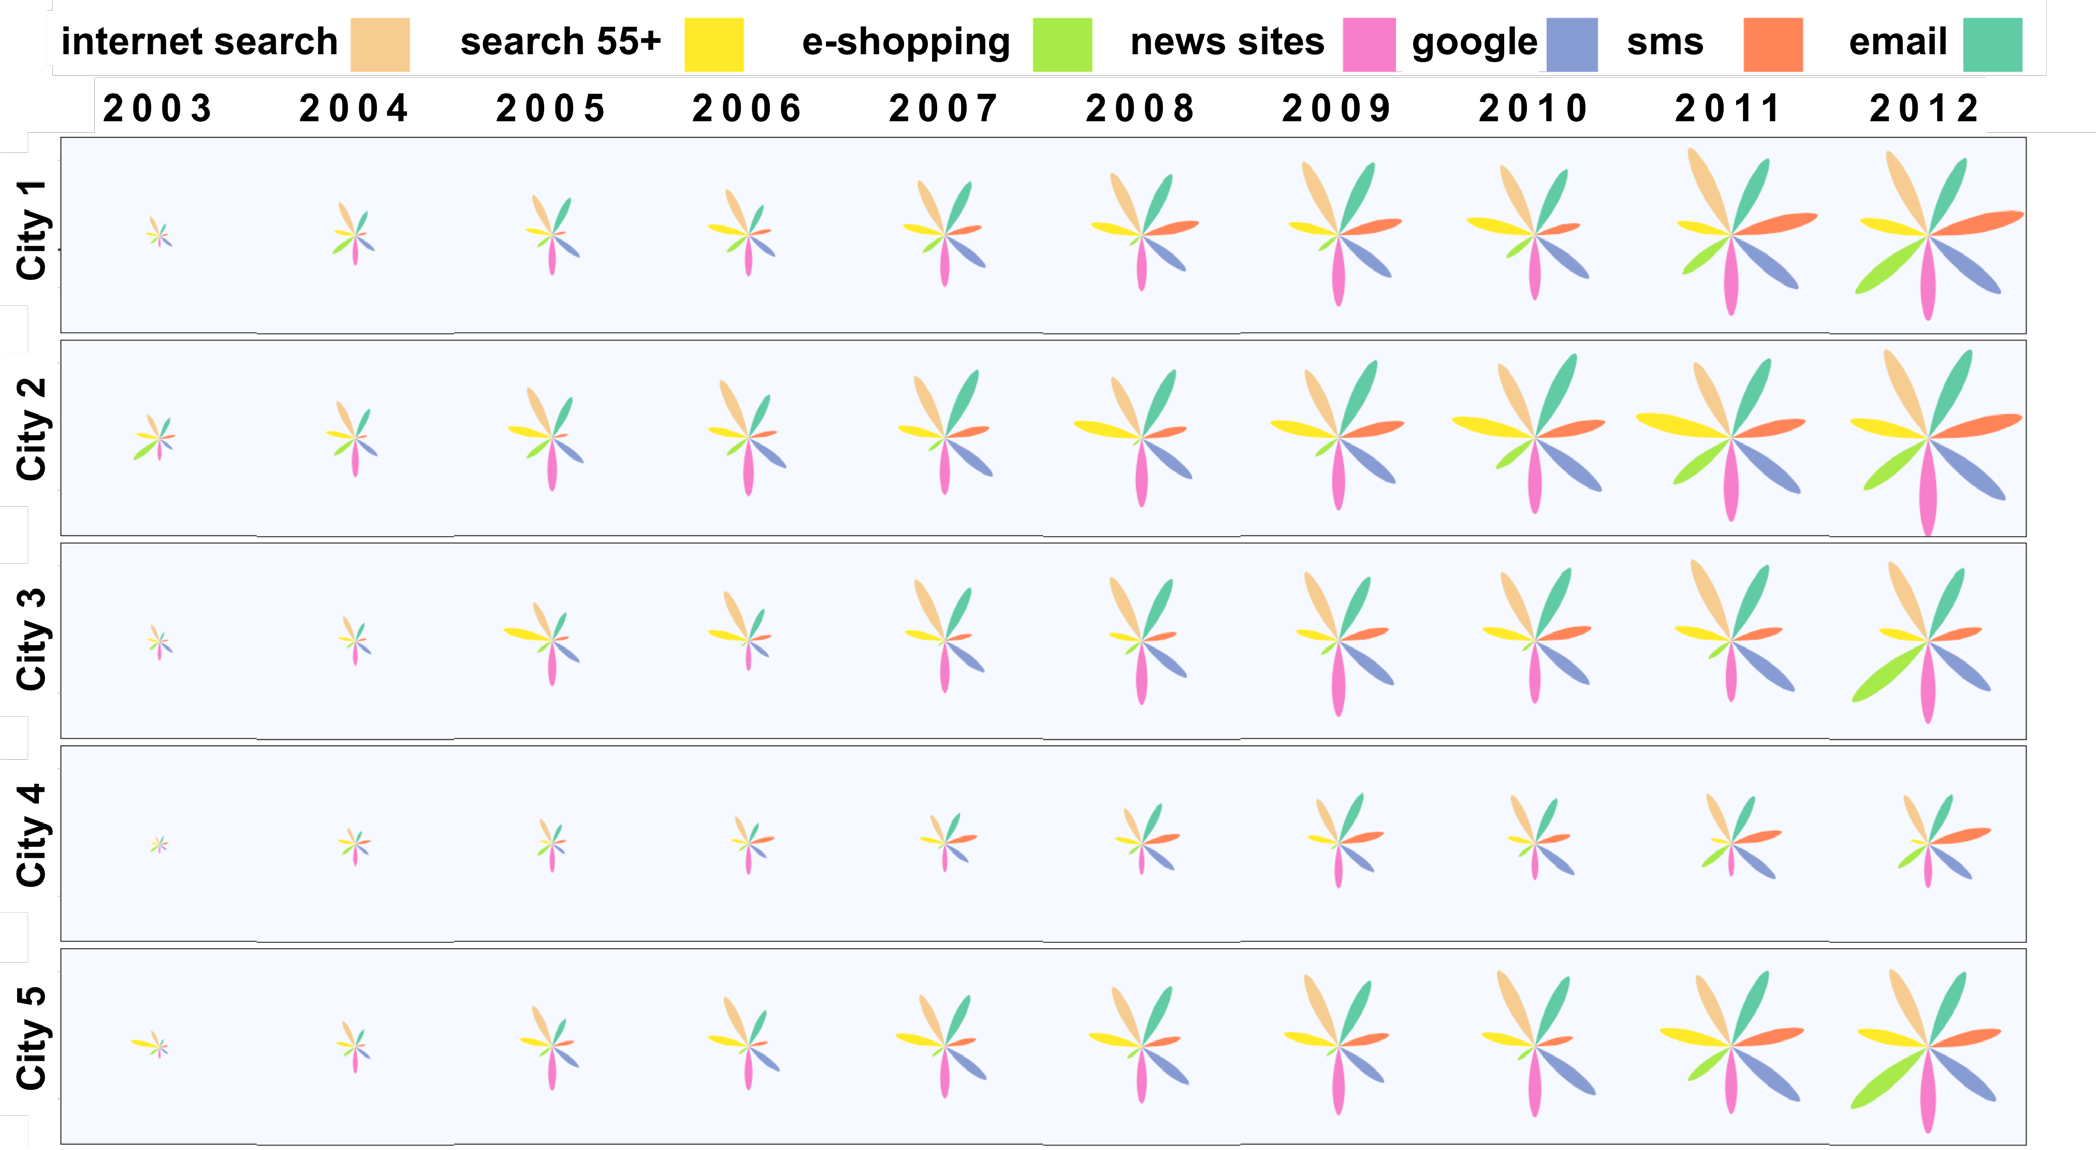
\includegraphics[scale=0.2]{flower.png}
    \caption{The size of each flower indicates Internet usage. The grid arrangement in this chart facilitates comparison both across time (horizontally) and city (vertically). As in figure~\ref{fig:radarchart}, Internet usage seems to conditionally dependent on time.}
    \label{fig:flowerchart}
    \end{subfigure}

    \bigskip
    \begin{subfigure}{\textwidth}
    \centering
    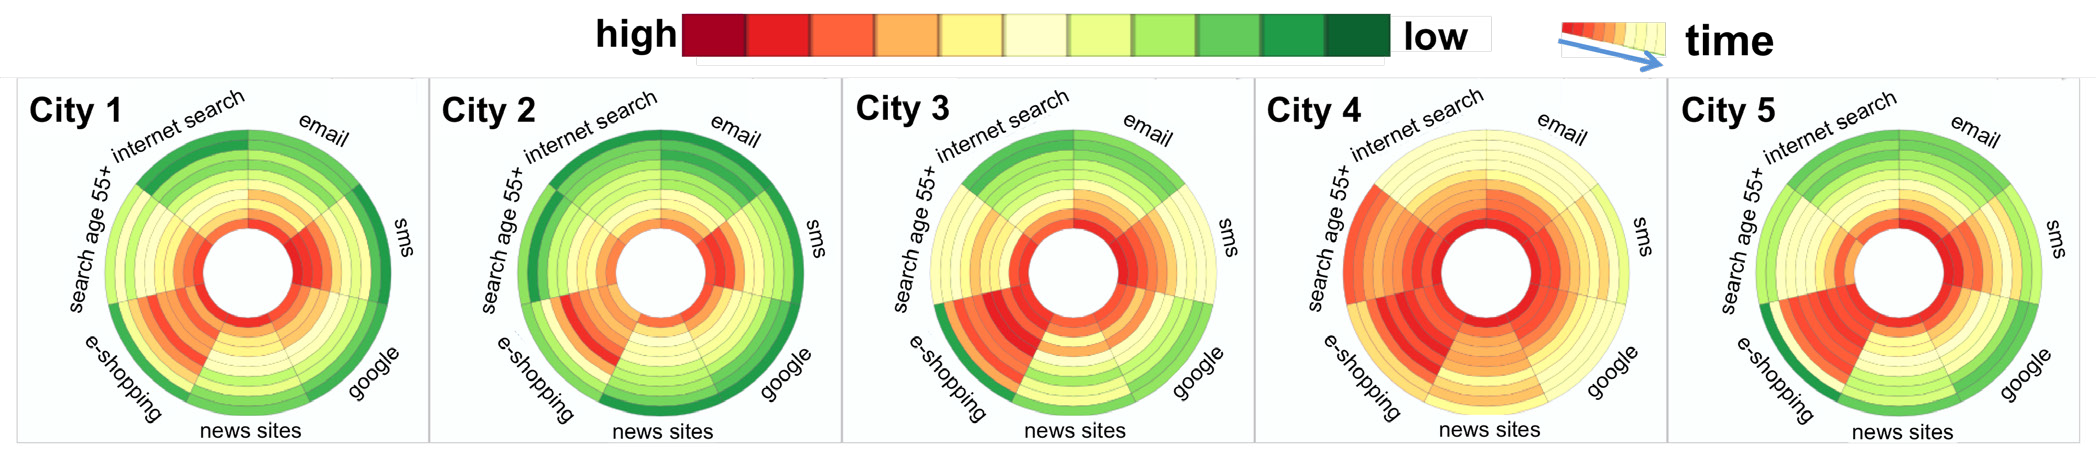
\includegraphics[scale=0.2]{circle.png}
    \caption{The circle chart prioritizes intensity of each type of usage, most clearly showing the popularity of shopping and SMS. This visualization facilitates testing a hypothesis of a conditional dependency amongst the Internet usage variables by isolating the similar pairwise color patterns in the presence and absence of a third usage type.}
    \label{fig:circlechart}
    \end{subfigure}
\caption{All three visualizations show Internet usage in 5 cities, from 2003 to 2012. Images are from Off the Radar: Comparative Evaluation of Radial Visualization Solutions for Composite Indicators \cite{albo_off_2016}}
\label{fig:radial}
\end{figure}
Radial visualizations are designed to show composite indicators (CI)\cite{chambers_graphical_1983}; a CI is a type of visualization wherein the multivariate observation is  mapped to a single visual idiom. For example, the whole line across all the Y-axis in a parallel coordinates plot (PCP) is a CI. A radar plot, as shown in figure~\ref{fig:radarchart}, is just a PCP where the two sides of the axis meet. Like a PCP, the radar chart shows pairwise relationships between variables that share nodes, but the radial shape also means it can show pairwise relationships between all variables. In 2010 in figure~\ref{fig:radarchart}, the more rectangular polygon for city 2 relative to the somewhat trapezoid polygon for city 4 indicate that Internet usage is characteristically different for the two cities. The conditional dependency factors in because the radial plot shows changes over time, by city, across multiple components of Internet usage. The flower chart in figure~\ref{fig:flowerchart} is very similar to the radar chart, also highlighting a potential dependency on time due to the use of small multiples and the flowers progressively getting larger. The circle chart in figure~\ref{fig:circlechart} stands out particularly because time progressions are not as readily visible, but instead this chart, especially with a finer grained colormap, best highlights the specific usage variables. This chart most clearly shows that shopping and sms seems to happen in tandem, and that clear color delineation also makes it easier for a user to scan the other variables to see how frequently they occur given the relationship between shopping and SMS. 

\subsubsection{Cluster Based Visualizations}
\begin{figure}
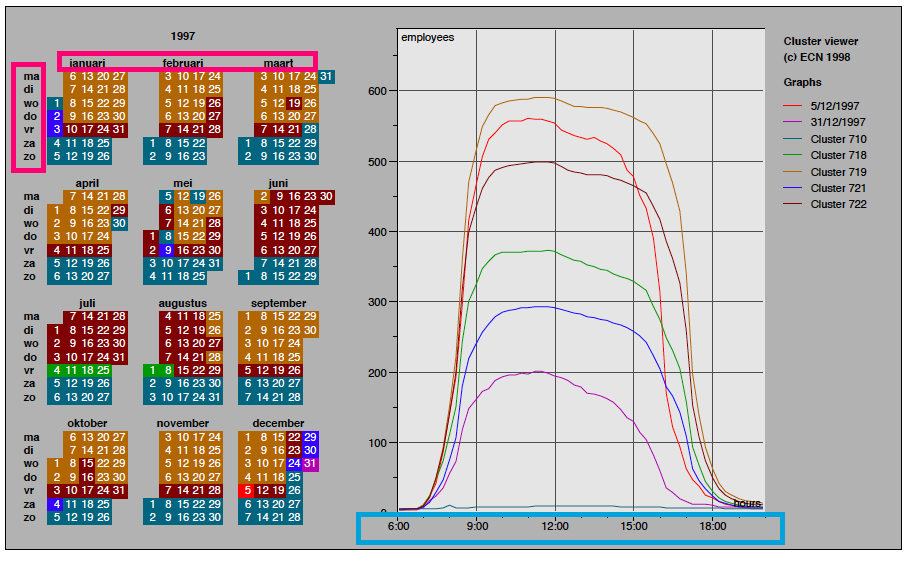
\includegraphics[width=1\textwidth]{calendar.png}
\caption{Figure from \cite{van_wijk_cluster_1999}. Van Wijk and Van Selow visualized the number of employees present at a research facility. This visualization shows that daily attendance seems to be more strongly dependent on day of week than time of day or day of the year. Figure is from Cluster and Calendar based Visualization of Time Series Data \cite{van_wijk_cluster_1999}}
\label{fig:calendar}
\end{figure}

Finding patterns and trends in large datasets, whether univariate or multivariate, is often a matter of trying to find representational fingerprints of common or outlying events in the dataset. This is frequently done through the use of a clustering algorithm. Figure~\ref{fig:calendar} shows an analysis of employee attendance at a research facility in the Netherlands\cite{van_wijk_cluster_1999}. Because the individual observations were recorded every 6 hours for a year, van Wilk and van Selow transformed the hourly observations into a matrix where each vector holds the observations for a given day. They then used an agglomerative clustering algorithm \cite{kaufman_agglomerative_1990} to find representative days, and color matched these clusters to a calendar of days to visualize how these clusters were distributed over time.  In this study, time is separated into three classes of events: time of day, day of week, and date. The researchers found that both the shape and magnitude of the attendance curve changed relative to the day of week, indicating a conditionally dependent relationship between attendance and day of week. 
\end{document}